% Author: Izaak Neutelings (June 2020)
% Inspiration:
%  https://courses.physics.ucsd.edu/2011/Summer/session1/physics2c/diffraction.pdf
%  https://tex.stackexchange.com/questions/201830/periodic-shading-in-tikz
\documentclass[border=3pt,tikz]{standalone}
\usepackage[outline]{contour} % glow around text
\usepackage{physics}
\usepackage{xcolor}
\usepackage{etoolbox} %ifthen
\usetikzlibrary{calc}
\usetikzlibrary{arrows,arrows.meta}
\usetikzlibrary{decorations.markings}
\usetikzlibrary{angles,quotes} % for pic (angle labels)
\usetikzlibrary{fadings}
\tikzset{>=latex} % for LaTeX arrow head
\contourlength{1.6pt}

\colorlet{wall}{blue!30!black}
\colorlet{myblue}{blue!70!black}
\colorlet{myred}{red!65!black}
\colorlet{mypurple}{red!50!blue!95!black!75}
\colorlet{myshadow}{blue!30!black!90}
\colorlet{mydarkred}{red!50!black}
\colorlet{mylightgreen}{green!60!black!70}
\colorlet{mygreen}{green!60!black}
\colorlet{myredgrey}{red!50!black!80}
\tikzstyle{wave}=[myblue,thick]
\tikzstyle{mydashed}=[black!70,dashed,thin]
\tikzstyle{mymeas}=[{Latex[length=3,width=2]}-{Latex[length=3,width=2]},thin]
\tikzstyle{mysmallarr}=[-{Latex[length=3,width=2]}]

\tikzset{
  declare function={
    int_arg(\y,\lam,\a,\L) = \a*\y/sqrt(\L*\L+\y*\y)/\lam; %sin(\x);
    int_one(\y,\lam,\a,\L) = (sin(180*int_arg(\y,\lam,\a,\L))/(pi*int_arg(\y,\lam,\a,\L)))^2;
    int_two(\y,\lam,\a,\L) = cos(180*int_arg(\y,\lam,\a,\L))^2;
    int_arg_ang(\t,\lam,\a) = \a*sin(\t)/\lam;
    int_one_ang(\t,\lam,\a) = (sin(180*int_arg_ang(\t,\lam,\a))/(pi*int_arg_ang(\t,\lam,\a)))^2;
    int_two_ang(\t,\lam,\a) = cos(180*int_arg_ang(\t,\lam,\a))^2;
  }
}

\newcommand\rightAngle[4]{
  \pgfmathanglebetweenpoints{\pgfpointanchor{#2}{center}}{\pgfpointanchor{#3}{center}}
  \coordinate (tmpRA) at ($(#2)+(\pgfmathresult+45:#4)$);
  \draw[white,line width=0.6] ($(#2)!(tmpRA)!(#1)$) -- (tmpRA) -- ($(#2)!(tmpRA)!(#3)$);
  \draw[mydarkred] ($(#2)!(tmpRA)!(#1)$) -- (tmpRA) -- ($(#2)!(tmpRA)!(#3)$);
}
\newcommand\lineend[2]{
  \def\w{0.1} \def\c{30}
  \draw[mygreen] (#1)++(#2:\w) to[out=#2-180-\c,in=#2+\c] (#1)
                               to[out=#2+\c-180,in=#2-\c]++ (#2-180:\w);
}
\def\tick#1#2{\draw[thick] (#1) ++ (#2:0.1) --++ (#2-180:0.2)}



\begin{document}


%% TWO SPLIT: interference x diffraction
%\begin{tikzpicture}
%  \def\A{3.5}
%  \def\d{3.4}     % slit distance
%  \def\a{0.9}     % slit size
%  \def\lambd{0.2} % wavelength
%  \def\k{15}      % x -> theta
%  \def\xmax{4.6}
%  \def\ymax{\A}
%  \def\N{4}
%  \def\D{2.3*\xmax}
%  \def\L{4.0}
%  \def\nsamples{80}
%  
%  \draw[->,thick,black] (-1.05*\xmax,0) -- (1.1*\xmax,0) node[below] {$\theta$};
%  \draw[->,thick,black] (0,-0.1*\A) -- (0,1.12*\A);
%  \draw[wave,variable=\t,samples=\nsamples,smooth,domain=-\xmax:\xmax]
%    plot(\t,{\A*int_one_ang(\k*\t,\lambd,\a)});
%  
%  \foreach \i [evaluate={\t=asin(\i*\lambd/\a)/\k;}] in {1,...,\N}{
%    \tick{-\t,0}{90} node[below=-1,scale=0.7] {$m=-\i$};
%    \tick{\t,0}{90} node[below=-1,scale=0.7] {$m=+\i$};
%  }
%  
%\end{tikzpicture}


% TWO SPLIT: interference x diffraction
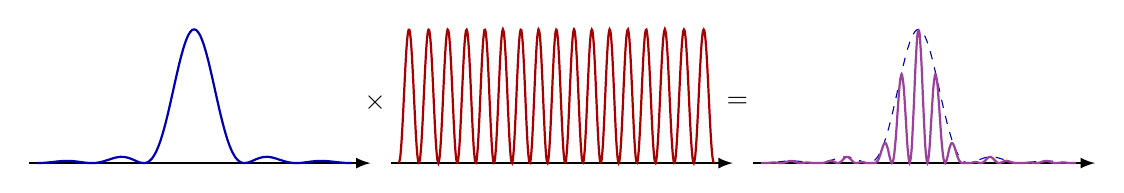
\begin{tikzpicture}
  \def\A{1.7}
  \def\d{3.4}     % slit distance
  \def\a{1.2}     % slit size
  \def\lambd{0.2} % wavelength
  \def\k{15}      % x -> theta
  \def\xmax{2}
  \def\D{2.3*\xmax}
  \def\L{4.0}
  \def\nsamples{80}
  
  % WAVE 1
  \draw[->,thick,black]
    (-1.05*\xmax,0) -- (1.12*\xmax,0);
  \draw[wave,variable=\t,samples=\nsamples,smooth,domain=-\xmax:\xmax]
    plot(\t,{\A*int_one_ang(\k*\t,\lambd,\a)});
  \node at (\D/2,0.45*\A) {$\times$};
  
  % WAVE 2
  \begin{scope}[shift={(\D,0)}]
    \draw[->,thick,black]
      (-1.05*\xmax,0) -- (1.12*\xmax,0);
    \draw[wave,myred,variable=\t,samples=3*\nsamples,smooth,domain=-\xmax:\xmax]
      plot(\t,{\A*int_two_ang(\k*\t,\lambd,\d)});
    \node at (\D/2,0.45*\A) {$=$};
  \end{scope}
  
  % WAVE 3
  \begin{scope}[shift={(2*\D,0)}]
    \draw[->,thick,black]
      (-1.05*\xmax,0) -- (1.12*\xmax,0);
    \draw[wave,dashed,thin,variable=\t,samples=\nsamples,smooth,domain=-\xmax:\xmax]
      plot(\t,{\A*int_one_ang(\k*\t,\lambd,\a)});
    \draw[wave,mypurple,variable=\t,samples=2*\nsamples,smooth,domain=-\xmax:\xmax]
      plot(\t,{\A*int_one_ang(\k*\t,\lambd,\a)*int_two_ang(\k*\t,\lambd,\d)});
  \end{scope}
  
\end{tikzpicture}


% DIFFRACTION - large slit - circular
\def\H{5.4}     % total wall height
\def\h{4.4}     % plane wave height
\def\t{0.18}    % wall thickness
\def\a{2.3}     % slit size
\def\lambd{0.4} % wavelength
\def\N{14}      % number of waves
\def\dN{30}     % number shift
\def\ang{6}    % angle of diffraction
\begin{tikzpicture}
  
  \def\lambd{0.4} % wavelength
  
  % WAVES
  \foreach \i [evaluate={\r=0.9*\i*\lambd;\R=(\i+\dN)*\lambd;}] in {1,...,\N}{
    \ifodd\i
      \draw[myblue,line width=0.8] (\r,{\R*sin(\ang)}) arc (\ang:-\ang:\R);
    \else
      \ifnumless{\i}{\N}{
        \draw[myblue!80,line width=0.1] (\r,{\R*sin(\ang)}) arc (\ang:-\ang:\R);
      }{}
    \fi
  }
  \foreach \i [evaluate={\xp=-2*(\i-0.5)*\lambd; \xm=-2*(\i-1)*\lambd;}] in {1,...,2}{
    \draw[myblue,line width=0.8] (\xp,-\h/2) -- (\xp,\h/2);
    \draw[myblue,line width=0.1] (\xm,-\h/2) -- (\xm,\h/2);
  }
  
  % WALL
  \fill[wall]
    (\t/2,\a/2) rectangle (-\t/2,\H/2)
    (\t/2,-\a/2) rectangle (-\t/2,-\H/2);
  
\end{tikzpicture}


% DIFFRACTION - large slit - straight
\def\ang{10} % angle of diffraction
\begin{tikzpicture}
  
  % WAVES
  \foreach \i [evaluate={\r=\i*\lambd;}] in {1,...,\N}{
    \ifodd\i
      \draw[myblue,line width=0.8] (\r,{\a/2+\r*sin(\ang)}) arc(\ang:0:\r) --++ (0,-\a) arc(0:-\ang:\r);
    \else
      \ifnumless{\i}{\N}{
        \draw[myblue,line width=0.1] (\r,{\a/2+\r*sin(\ang)}) arc(\ang:0:\r) --++ (0,-\a) arc(0:-\ang:\r);
      }{}
    \fi
  }
  \foreach \i [evaluate={\xp=-2*(\i-0.5)*\lambd; \xm=-2*(\i-1)*\lambd;}] in {1,...,2}{
    \draw[myblue,line width=0.8] (\xp,-\h/2) -- (\xp,\h/2);
    \draw[myblue,line width=0.1] (\xm,-\h/2) -- (\xm,\h/2);
  }
  
  % WALL
  \fill[wall]
    (\t/2,\a/2) rectangle (-\t/2,\H/2)
    (\t/2,-\a/2) rectangle (-\t/2,-\H/2);
  
\end{tikzpicture}


% DIFFRACTION - obstacle - straight
\begin{tikzpicture}
  
  % WAVES
  \foreach \i [evaluate={\r=\i*\lambd;}] in {1,...,\N}{
    \ifodd\i
      \draw[myblue,line width=0.8]
        (\r,\H/2) -- (\r,0.5*\a) arc (0:-\ang:\r)
        (\r,-\H/2) -- (\r,-0.5*\a) arc (0:\ang:\r);
    \else
      \ifnumless{\i}{\N}{
        \draw[myblue!80,line width=0.1]
          (\r,\H/2) -- (\r,0.5*\a) arc (0:-\ang:\r)
          (\r,-\H/2) -- (\r,-0.5*\a) arc (0:\ang:\r);
      }{}
    \fi
  }
  \foreach \i [evaluate={\xp=-2*(\i-0.5)*\lambd; \xm=-2*(\i-1)*\lambd;}] in {1,...,2}{
    \draw[myblue,line width=0.8] (\xp,-\H/2) -- (\xp,\H/2);
    \draw[myblue,line width=0.1] (\xm,-\H/2) -- (\xm,\H/2);
  }
  
  % WALL
  \fill[wall] (-\t/2,-\a/2) rectangle (\t/2,\a/2);
  
\end{tikzpicture}


% DIFFRACTION - small slit
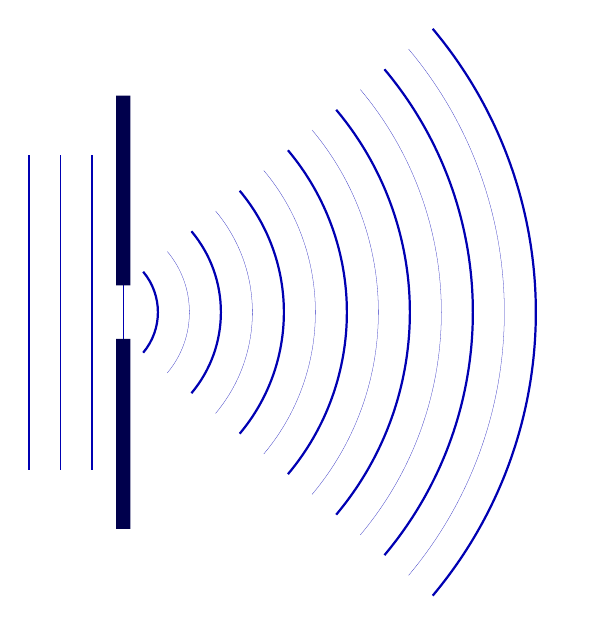
\begin{tikzpicture}
  
  \def\H{5.5}     % total wall height
  \def\h{4.0}     % plane wave height
  \def\t{0.18}    % wall thickness
  \def\a{0.68}    % slit distance
  \def\N{7}       % number of waves
  \def\lambd{0.4} % wavelength
  \def\ang{40}
  
  % WAVES
  \foreach \i [evaluate={\Rp=2*\i*\lambd; \Rm=2*(\i+0.5)*\lambd;}] in {1,...,\N}{
    \draw[myblue,line width=0.8] (-0.9*\lambd,0)++(\ang:\Rp) arc (\ang:-\ang:\Rp);
    \ifnumless{\i}{\N}{
      \draw[myblue!80,line width=0.1] (-0.9*\lambd,0)++(\ang:\Rm) arc (\ang:-\ang:\Rm);
    }{}
  }
  \foreach \i [evaluate={\xp=-2*(\i-0.5)*\lambd; \xm=-2*(\i-1)*\lambd;}] in {1,...,2}{
    \draw[myblue,line width=0.8] (\xp,-\h/2) -- (\xp,\h/2);
    \draw[myblue,line width=0.1] (\xm,-\h/2) -- (\xm,\h/2);
  }
  
  % WALL
  \fill[wall]
    (\t/2,\a/2) rectangle (-\t/2,\H/2)
    (\t/2,-\a/2) rectangle (-\t/2,-\H/2);
  
\end{tikzpicture}


% DIFFRACTION - ONE SLIT - projection
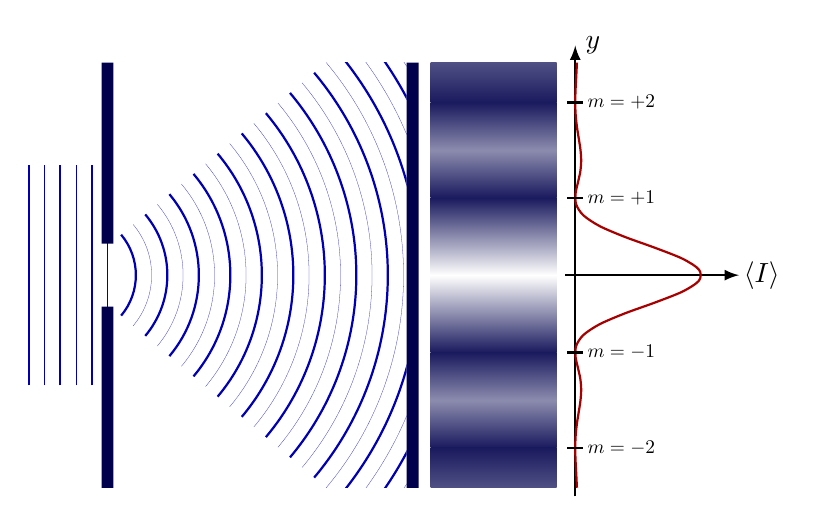
\begin{tikzpicture}[
    nodal/.style={mylightgreen,dashed,very thin},
  ]
  
  \def\L{3.8}       % distance between walls
  \def\H{5.4}       % total wall height
  \def\h{2.8}       % plane wave height
  \def\t{0.15}      % wall thickness
  \def\a{0.8}       % slit distance
  \def\d{0.20}      % slit size
  \def\N{21}        % number of waves
  \def\dN{1}        % shift radius
  \def\A{1.6}       % amplitude
  \def\lambd{0.20}  % wavelength
  \def\R{\N*\lambd} % wave radius
  \def\Nfringes{2}  % number of nodal lines
  \def\nsamples{40}
  \def\ang{40}
  
  % PLANE WAVES
  \foreach \i [evaluate={\xp=-2*(\i-0.5)*\lambd; \xm=-2*(\i-1)*\lambd;}] in {1,...,3}{
    \draw[myblue,line width=0.8] (\xp,-\h/2) -- (\xp,\h/2);
    \draw[myblue,line width=0.1] (\xm,-\h/2) -- (\xm,\h/2);
  }
  
  % WAVES
  \begin{scope}
    \clip (-\t/2,-\H/2) rectangle (\L,\H/2);
    \foreach \i [evaluate={\Rp=2*(\i+\dN)*\lambd; \Rm=2*(\i+\dN+0.5)*\lambd;}] in {1,...,\N}{
      \draw[myblue,line width=0.8] (-2.2*\lambd,0)++(\ang:\Rp) arc (\ang:-\ang:\Rp);
      \draw[myblue!80,line width=0.1] (-2.2*\lambd,0)++(\ang:\Rm) arc (\ang:-\ang:\Rm);
    }
  \end{scope}
  
  % WALL
  \fill[wall]
    (\t/2,\a/2) rectangle (-\t/2,\H/2)
    (\t/2,-\a/2) rectangle (-\t/2,-\H/2)
    (\L,-\H/2) rectangle (\L+\t,\H/2);
  
  % SHADES
  \begin{scope}[shift={(1.08*\L,0)}]
    \clip (0,-\H/2) rectangle (1.1*\A,\H/2);
    \def\yz{\L/sqrt((\a/\lambd)^2-1)} %\L/sqrt((\a/\lambd)^2-1)
    \path [left color=myshadow,right color=myshadow,middle color=white,shading angle={180}]
      (0,{-\yz}) rectangle (\A,{\yz});
    \foreach \i [evaluate={
                  \n=\i;
                  \m=\i+1;
                  \yn=\L/sqrt((\a/(\lambd*\n))^2-1); %\L*\n*\lambd/\a
                  \ym=\L/sqrt((\a/(\lambd*\m))^2-1);
                  \dang=mod(\i,2)*180;
                 }] in {1,...,\Nfringes}{
      \path [left color=myshadow,right color=myshadow,middle color=myshadow!50,shading angle={\dang}]
        (0,\yn) rectangle (\A,\ym);
      \path [left color=myshadow,right color=myshadow,middle color=myshadow!50,shading angle={180+\dang}]
        (0,-\yn) rectangle (\A,-\ym);
    }
  \end{scope}
  
  % INTENSITY
  \begin{scope}[shift={(1.1*\L+1.1*\A,0)}]
    \draw[->,thick] (-0.08*\A,0) -- (1.3*\A,0) node[right=-2] {$\expval{I}$};
    \draw[->,thick] (0,-0.52*\H) -- (0,0.54*\H) node[right] {$y$};
    \draw[myred,thick,variable=\y,samples=\nsamples,smooth,domain=-\H/2:\H/2]
      plot({\A*int_one(\y,\lambd,\a,\L)},\y);
    \foreach \i [evaluate={\y=\L/sqrt((\a/(\lambd*\i))^2-1);}] in {1,...,\Nfringes}{
      \tick{0,-\y}{180} node[right=-1,scale=0.7] {$m=-\i$};
      \tick{0,\y}{180} node[right=-1,scale=0.7] {$m=+\i$};
    }
  \end{scope}
  
\end{tikzpicture}


% DIFFRACTION - ONE SLIT - PATH DIFFERENCE
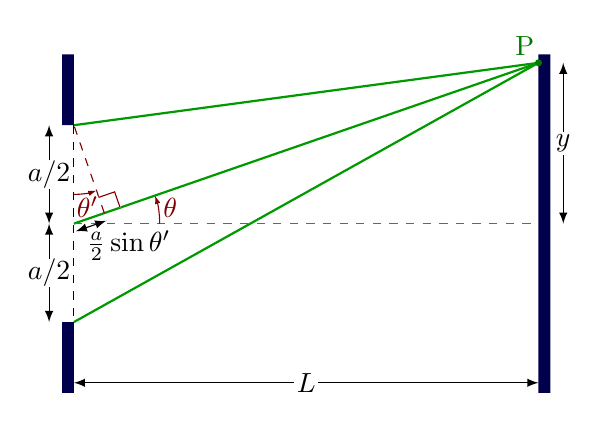
\begin{tikzpicture}
  
  \def\L{5.9}       % distance between walls
  \def\H{4.3}       % total wall height
  \def\f{0.95}      % fractional height of projection point
  \def\ang{atan((\f*\H+\a/2)/\L/2)} % theta
  \def\t{0.15}      % wall thickness
  \def\a{2.5}       % slit distance
  \coordinate (T) at (0,\a/2);
  \coordinate (B) at (0,-\a/2);
  \coordinate (L) at (0,0);
  \coordinate (R) at (\L,0);
  \coordinate (P) at (\L,\f*\H/2);
  \coordinate (M) at ($(L)!(T)!(P)$);
  
  % LINES
  \draw[mygreen,thick] (T) -- (P); %node[midway,above=-1] {$r_1$};
  \draw[mygreen,thick] (B) -- (P); %node[midway,below=3,right=6] {$r_2$}; %right=6,below right=-4
  \draw[mygreen,thick] (L) -- (P);
  \draw[dashed] (T) -- (B);
  \draw[dashed,black!60] (L) -- (R);
  \draw[mydarkred,dashed] (M) -- (T);
  
  % ANGLES
  \draw pic[mysmallarr,"$\theta'$",mydarkred,draw=mydarkred,angle radius=25,angle eccentricity=1.2]
    {angle = B--T--M};
  \draw pic[mysmallarr,"$\theta$",mydarkred,draw=mydarkred,angle radius=31,angle eccentricity=1.14]
    {angle = R--L--P};
  \rightAngle{T}{M}{P}{0.3}
  
  % MEASURES
  \draw[<->,black] (0,-0.47*\H) --++ (\L,0) node[midway,fill=white,inner sep=1] {$L$};
  \draw[<->,black] (-2.1*\t,0) --++ (0,\a/2) node[midway,fill=white,inner sep=0.1] {$a/2$};
  \draw[<->,black] (-2.1*\t,0) --++ (0,-\a/2) node[midway,fill=white,inner sep=0.1] {$a/2$};
  \draw[<->,black] ([shift={({\ang-100}:0.1)}]L) -- ([shift={({\ang-100}:0.1)}]M)
    node[midway,left=3,below right=-2]{$\frac{a}{2}\sin\theta'$};
  \draw[<->,black] ([shift={(2.1*\t,0)}]P) -- ([shift={(2.1*\t,0)}]R)
    node[midway,fill=white,inner sep=1]{$y$};
  
  % WALL
  \fill[wall]
    (0,\a/2) rectangle (-\t,\H/2)
    (0,-\a/2) rectangle (-\t,-\H/2)
    (\L,-\H/2) rectangle (\L+\t,\H/2);
  \fill[mygreen!80!black] (P) circle (0.3*\t) node[right=1,above left=-1] {P};
  
\end{tikzpicture}


% DIFFRACTION - ONE SLIT - PATH DIFFERENCE close up
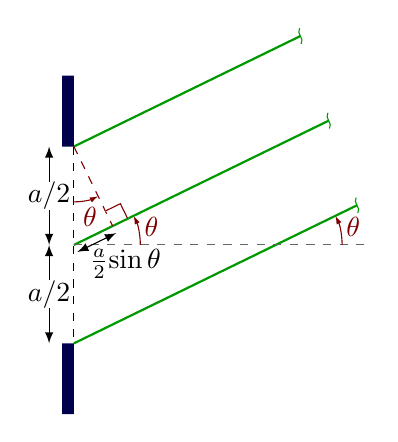
\begin{tikzpicture}
  
  \def\L{6.15}      % distance between walls
  \def\l{4.0}       % path length
  \def\H{4.3}       % total wall height
  \def\f{0.9}       % fractional height of projection point
  \def\t{0.15}      % wall thickness
  \def\a{2.5}       % slit distance
  \def\ang{26}      % angle
  \coordinate (T) at (0,\a/2);
  \coordinate (B) at (0,-\a/2);
  \coordinate (L) at (0,0);
  \coordinate (R) at (\L,0);
  \coordinate (I) at ({\a/2/tan(\ang)},0);
  
  % LINES
  \draw[mygreen,thick] (T) --++ (\ang:.8*\l) coordinate (PT); %node[midway,below=1,above left=-2] {$r_1$};
  \draw[mygreen,thick] (B) --++ (\ang:\l) coordinate (PB); %node[midway,left=2,below right=-1] {$r_2$};
  \draw[mygreen,thick] (L) --++ (\ang:.9*\l) coordinate (PR);
  \draw[dashed] (T) -- (B);
  \draw[mydarkred,dashed] (T) -- ($(L)!(T)!(PR)$) coordinate (M);
  %\draw[black!60,dashed] (T) --++ (.20*\L,0) coordinate (TR);
  \draw[black!60,dashed] (L) --++ (.6*\L,0) coordinate (LR);
  %\draw[black!60,dashed] (B) --++ (.20*\L,0) coordinate (BR);
  
  % LINE END
  \lineend{PT}{\ang+70}
  \lineend{PR}{\ang+70}
  \lineend{PB}{\ang+70}
  
  % ANGLES
  \draw pic[mysmallarr,"$\theta$",mydarkred,draw=mydarkred,angle radius=20,angle eccentricity=1.3]
    {angle = B--T--M}; %\contour{white}{}
  \draw pic[mysmallarr,"$\theta$",mydarkred,draw=mydarkred,angle radius=24,angle eccentricity=1.2]
    {angle = LR--L--PR};
  \draw pic[mysmallarr,"$\theta$",mydarkred,draw=mydarkred,angle radius=24,angle eccentricity=1.2]
    {angle = LR--I--PB};
  \rightAngle{T}{M}{PR}{0.3}
  
  % MEASURES
  \draw[<->,black] (-2.1*\t,0) --++ (0,\a/2) node[midway,fill=white,inner sep=0.1] {$a/2$};
  \draw[<->,black] (-2.1*\t,0) --++ (0,-\a/2) node[midway,fill=white,inner sep=0.1] {$a/2$};
  \draw[<->,black] ([shift={({\ang-90}:0.1)}]L) -- ([shift={({\ang-90}:0.1)}]M)
    node[midway,left=5,below right=-1]{$\frac{a}{2}\!\sin\theta$};
  
  % WALL
  \fill[wall]
    (0,\a/2) rectangle (-\t,\H/2)
    (0,-\a/2) rectangle (-\t,-\H/2);
  
\end{tikzpicture}



\end{document}